\documentclass[../zhang_thesis.tex]{subfiles}
\begin{document}

\chapter{Methodology}

%%%%%%%%%%%%%%%%%%%%%%%%%%%%%%%%%%%%%%%%%%%%%%%%%%%%%%%%%%%%%%%

\section{Battery Model}

As discussed in the previous section, this thesis considers the electrical-circuit battery model proposed by Chen and Rinc\'on-Mora~\cite{chen06} and shown in \autoref{fig:batt_model}. The left portion of the circuit models the capacity, SOC, and runtime, while the right portion models the transient i-v characteristics.  For convenience, the model is designed so that the SOC of the battery equals the voltage $V_\text{SOC}$, in volts. The parameters $C_\text{cap}$ and $R_{sd}$ are assumed constant
for a given battery and determine the capacity and self-discharge rate of the battery. The other parameters are all nonlinear functions of $V_\text{SOC}$ and determine the transient i-v response as well as the open-circuit voltage $V_\text{OC}$. From a typical TCL PL-383562 polymer lithium-ion battery, Chen and Rinc\'on-Mora extracted these parameters and fit them to curves, obtaining
\begin{gather}
	R_s(V_\text{SOC}) = 0.1562 e^{-24.37 V_\text{SOC}} + 0.07446 \\
	R_{ts}(V_\text{SOC}) = 0.3208 e^{-29.14 V_\text{SOC}} + 0.04669 \\
	C_{ts}(V_\text{SOC}) = -752.9 e^{-13.51 V_\text{SOC}} + 703.6 \\
	R_{tl}(V_\text{SOC}) = 6.603 e^{-155.2 V_\text{SOC}} + 0.04984 \\
	C_{tl}(V_\text{SOC}) = -6056 e^{-27.12 V_\text{SOC}} + 4475 \\
	V_\text{OC}(V_\text{SOC}) = -1.031 e^{-35 V_\text{SOC}} + 3.685 + 0.2156 V_\text{SOC} - 0.1178 V_\text{SOC}^2 + 0.3201 V_\text{SOC}^3
\end{gather}
The resistance and capacitance parameters shown above are approximately constant for $\text{SOC}>0.2$ and change exponentially for $\text{SOC}<0.2$. The open-circuit voltage also changes exponentially for $\text{SOC}<0.2$ but is approximately linear for $\text{SOC}>0.2$.

\begin{figure}[ht]
\centering
\includegraphics[width=0.9\textwidth]{batt_model}
\caption{Battery model for simulation. [From paper, will redo later]}
\label{fig:batt_model}
\end{figure}

This study used the nonlinear parameters given by Chen and Rinc\'on-Mora for the implementation of a battery using their battery model in Matlab. \emph{The other, constant parameters were chosen to produce a capacity of 4~Ah and a self-discharge rate of 4\% per month, assuming a nominal voltage of 3.7~V. [I didn't properly derive the following equations so my actual values are different.]} To do so, the equivalent capacitance $C_\text{cap}$ to deliver the desired capacity is calculated, and then the resistance $R_{sd}$
that produces the desired self-discharge rate is calculated. More specifically, the capacitance $C_\text{cap}$ is chosen to so that it supplies the same energy as a battery when discharged at
\begin{equation}
    I_t\,[\text{A}] = C_n\,[\text{Ah}] / 1\,[\text{h}],
\end{equation}
where $I_t$ is the discharge current in amperes, $C_n$ is the rated capacity in ampere-hours, and $n$ is the time base in hours for which the rated capacity is declared~\cite{iec61434,linden01_ch3}. Note that by definition, a fully charged battery with capacity $C_n$ is fully discharged in $n$ hours when discharged at a constant current of $I_t/n$~\cite{linden01_ch3}. The energy delivered by the battery over the $T=n$~hours is then
\begin{align}
    E_\text{batt} &= \int_0^T V(t) I(t) \,\mathrm{d}t = T \left( \frac{1}{T} \int_0^T V(t)\,\mathrm{d}t \right) \frac{I_t}{n} = V_n I_t (1\,\text{h}) \\
    &= 3600 V_n I_t (\text{s}) \,[\text{J}],
\end{align}
where $V_n$ is the nominal voltage. The energy stored in the capacitor $C_\text{cap}$ is $E_\text{cap} = C_\text{cap} V_\text{SOC,max}^2 / 2$. Recall that $V_\text{SOC}$ has a maximum voltage of 1~V, so the capacitance needs to be
\begin{equation}
    C_\text{cap} = 2E_\text{batt}/(1\,\text{V}^2) = 7200 V_n I_t (\text{s}/\text{V}^2) \,[\text{F}]
\end{equation}
Then, the resistance $R_{sd}$ is chosen so that the time constant $\tau=RC$ results in the desired drop of $\xi=0.04$ over $T=1$~month as follows
\begin{gather}
    V(t) = V_0 e^{-T/\tau} = V_0 (1-\xi) \\
    \tau = -T/\ln(1-\xi) = -2592000/\ln 0.96 \,[\text{s}].
\end{gather}
Then, $R_{sd}=\tau/C_\text{cap}$. Thus, the parameters are $C_\text{cap}=106.56$~kF and $R_{sd}=595.86~\Omega$. \emph{[Actual values used in study are $C=3789.5$ and $R=6290.7$. That works out to 1422.5~mAh and 10.3\% per month. Question is whether to change original setup or redo simulations.]}

For ease of filter design, it is useful to derive the state-space representation of the battery model. The physical variable definition is used, where the state variables are chosen to represent the stored charge in each capacitor. Choosing $x_1=C_{ts}V_{ts}$, $x_2=C_{tl}V_{tl}$, and $x_3=C_\text{cap}V_\text{SOC}$, where the voltages are as defined in \autoref{fig:batt_model}, achieves the goal. Additionally, it can be seen that the cell current influences the state variables, while the
cell voltage is influenced by them. Therefore, $i_\text{cell}$ is defined as the state input and $V_\text{cell}$ is defined as the state output. The resulting state space representation is
\begin{gather}
    \dot{\mathbf{x}} = \begin{bmatrix}
        -1/R_{ts}C_{ts} & 0 & 0 \\
        0 & -1/R_{tl}C_{tl} & 0 \\
        0 & 0 & -1/R_{sd}C_\text{cap}
    \end{bmatrix} \mathbf{x} + \begin{bmatrix} 1 \\ 1 \\ -1 \end{bmatrix} i_\text{cell} \\
    V_\text{cell} = V_\text{OC} - \frac{x_1}{C_{ts}} - \frac{x_2}{C_{tl}} - R_s i_\text{cell}.
\end{gather}
While the above appears to be a linear system, remember that many of the parameters are functions of $V_\text{SOC}$, and thus, depend on the state $x_3$. Therefore, this is a nonlinear system.

%To better determine the necessity of nonlinear filtering for thus system, it is useful to determine the degree of nonlinearity. Recent work in quantizing the degree of nonlinearity was conducted by

\section{Filter Implementations}

%As was seen in the last section, the degree of nonlinearity of the battery model necessitates the use of a nonlinear filter. However, for SOC$>0.2$, the dynamics behave approximately linearly, because the resistance and capacitance parameters are approximately constant. Since the battery operates in this ``linear'' region for the majority of the time, it is useful to compare the performance of a linear filter to the nonlinear filters discussed in \autoref{sec:nl_filt}.

%In order to determine the necessity of incorporating the nonlinear relationship between $V_\text{SOC}$ and $V_\text{OC}$ in the filter design, the linearized right-hand circuit with $V_\text{SOC}=0.6$~V and the left-hand circuit were processed by a Kalman filter in each iteration and in that order, with the nonlinearity calculated implicitly.
% the left-hand circuit along with the right-hand circuit linearized at $V_\text{SOC}=0.6$~V were consecutively processed by the Kalman filter in each itera

\section{Simulation Setup}

\begin{figure}
\centering
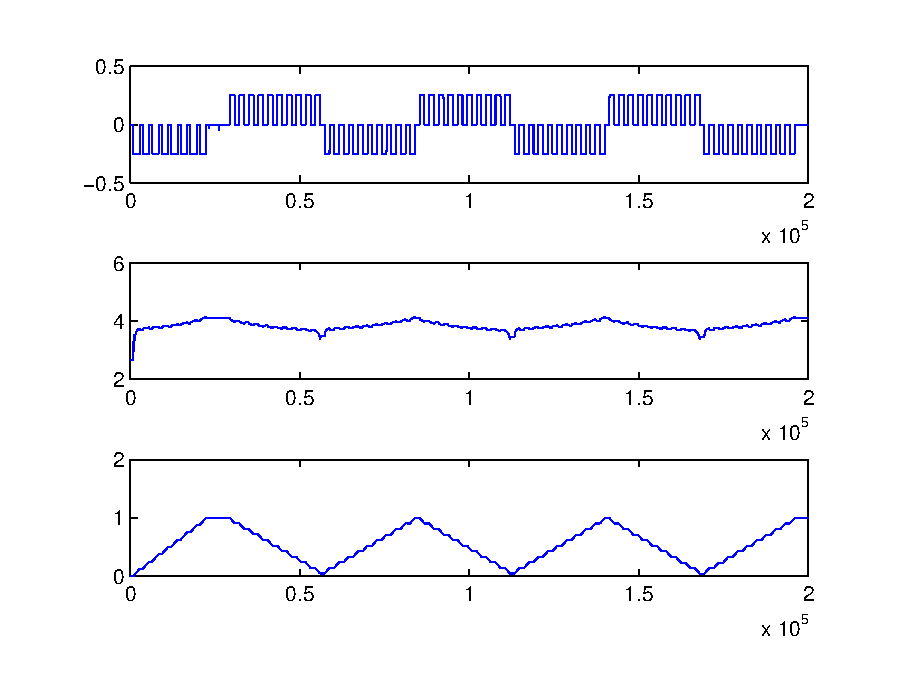
\includegraphics[width=0.9\textwidth]{sim_ideal}
\caption{Discharge current along with the resulting voltage and SOC.}
\label{fig:idealsim}
\end{figure}

\end{document}
